\section{I/O Automata Component Model\label{component_model}}

%% Modularity, well-defined interfaces, and composition are essential properties of reusable software.
%% A unit of software that exhibits all of these properties is called a \emph{component}~\cite{szyperski2002component}.
%% Modularity implies that a component can be deployed independently of other components.
%% Well-defined interfaces and interactions allow components to expose their functionality in a regular way that facilitates reasoning about different interactions among them.
%% Composition allows a group of interacting components to be understood as a cohesive unit.

In this section we describe how the I/O automata model offers a natural realization of components and interfaces, and provides natural support for concurrency and composition.
%% We then describe extensions to support dynamic semantics as participants in the system may arrive and depart at run-time.
We then describe extensions to support semantics for \emph{dynamic systems,} i.e., systems whose set of constituent automata changes over time.

\paragraph*{I/O automata.}
The Input/Output (I/O) automata model was developed to model reactive concurrent and asynchronous systems~\cite{lynch1996distributed}.
An I/O automaton consists of state variables and a set of atomic actions that manipulate the state variables.
An action is only permitted to manipulate the state variables of the automaton to which it belongs.
An action is either an internal action, an output action, or an input action.
An internal action only changes the state of the automaton.
An output action changes the state of the automaton and produces a signal or value that may be consumed by one or more input actions.
An input action changes the state of the automaton when it receives a signal or value produced by an output action.
\ifjournal
The set of actions associated with an automaton is known as the automaton's \emph{signature}~\cite{lynch1996distributed}.
\fi
\ifjournal
Often, a local action consists of a precondition and an effect.
The precondition is a predicate over the state variables that enables the effect when selected for execution.
The effect is a function that computes the next state of the automaton from the current state.
An input action presented in this style consists solely of an effect.
\fi
I/O automata are \emph{composed} by (1)~concatenating the state variables of the constituent automata, (2)~consolidating the effects of all input actions with the same name, and (3)~incorporating the effects of input actions into output actions with the same name.
Execution in the I/O automata model consists of non-deterministically and repeatedly selecting a local action (an output or internal action~\cite{lynch1996distributed}) and then if the precondition is true applying the effect.
The scheduler is assumed to be \emph{fair,} meaning that a local action is guaranteed to be selected (but not necessarily executed) infinitely often.

\begin{figure*}
\center
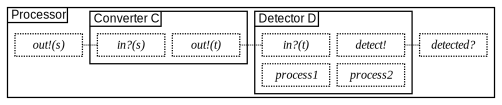
\includegraphics[width=\textwidth]{system_model}
\caption{Example event detection system.}
\label{sys_model}
\end{figure*}

\paragraph*{Motivation for I/O automata based components.}
%The I/O automata formalism was developed to model reactive systems~\cite{lynch1987hierarchical} and has been used in the design and verification of concurrent and distributed systems.
I/O automata are a good foundation for such components because they have independent state, straightforward interfaces, and precise semantics for event generation, distribution, and consumption resulting in well-defined interactions under composition.
\emph{Hierarchical decomposition} is an established technique for I/O automata~\cite{lynch1994atomic} which allows a \emph{parent} to contain zero or more \emph{children}.
The \emph{root automaton} is the automaton at the top of the hierarchy and represents the entire system as composition is applied recursively up the hierarchy.

To illustrate how components can be expressed naturally using I/O automata, Figure~\ref{sys_model} shows a simple event detector system comprising three component automata: an anonymous Processor, a Converter named C, and a Detector named D. 
The Processor automaton is the root and C and D are its children.
Automata are depicted as solid rectangles. The type of the automaton appears in a box in the upper left or lower left corner, e.g., Processor.
The name of a named automaton appears after its type, e.g., Converter C.
Actions are depicted as dotted rectangles and bindings are indicate by dotted lines with an arrow pointing to the input action.
Output actions are suffixed with \emph{!} (e.g., \emph{detect!}), input actions are suffixed with \emph{?} (e.g., \emph{detected?}), and internal actions have neither suffix (e.g., \emph{process1}).
The type associated with the value produced or consumed by an action is in parentheses after the name (e.g., \emph{out!(s)}).

\paragraph*{Explicit composition.}
Composition of I/O automata is based on actions having the same name.
To prepare for dynamic composition, we redefine composition at the action level.
An explicit association between an output action and input action is called a \emph{binding}.
%% The automaton that prescribes a binding is said to \emph{own} the binding.
%% A binding is denoted $(output, input, owner)$.
The set of bindings in a system must adhere to four essential rules.
First, the output action and input action of a binding must agree on the type being produced and consumed.
Second, an input action can be bound to at most one output action.
Third, an output action cannot be bound to more than one input action in the same automaton.
Fourth, an output action cannot be bound to an input action in the same automaton.
The second, third, and fourth rules exist because they admit ambiguity into the relationship between the states of the associated automata.
Graphically, an arrow originating in one component automaton must terminate in another component automaton as Figure~\ref{sys_model} illustrates.
%% To adhere to this rule, the following must be true for the global binding map $B$:  $\langle \forall o, i : (o, i) \in B :: \pi (o) \neq \pi (i) \rangle$.

\paragraph*{Concurrent execution.}
Since the state of each automaton is independent, opportunities exist for concurrent execution if the state of each automaton is preserved and a composition is not reduced to a single equivalent automaton.
Each local action implies a set of automata which in turn implies a set of state variables that might be modified.
For an internal action, this set consists of the automaton containing the internal action.
For an output action, this set consists of the automaton containing the output action and the automata that contain the input actions to which the output action is bound.
Two actions can be executed concurrently if their respective sets of state variables are disjoint.
The implied automata sets for each local action in Figure~\ref{sys_model} are: $out!(s) \to \{root, C\}$, $out!(t) \to \{C, D\}$, $process1 \to \{D\}$, $process2 \to \{D\}$, and $detect! \to \{D, root\}$.
Thus, $out!(s)$ and $process1$ can be executed concurrently while $process1$ and $detect!$ can not.

\ifjournal
These observations create some interesting opportunities for designing and analyzing concurrent software.
Migrating intense computation to internal actions increases the level of parallelism in a system, i.e., the set of implied automata is small.
A high degree of fan-out (an output action being bound to many input actions) creates a bottle-neck and decreases the level of parallelism, i.e., the set of implied automata is large.
However, the input effects can be applied in parallel since the state of each automaton is independent.
A high degree of fan-in (an automaton has many bound input actions) also creates a bottle-neck by increasing the probability that two sets of implied automata will not be disjoint.
A scheduler might cluster and pin automata to processors to maximize concurrent execution while minimizing inter-processor communication.
Compositions of automata can be statically composed to take advantage of in-lining.
An individual automaton can be decomposed into a number of child automata to increase parallelism.

\paragraph*{Parameters and action types.}
Actions in the I/O automata model can be defined using parameters.
Parameters are useful for situations requiring fan-in or session semantics.
For example, consider an automaton with an input action $in?(s)$ that is to be bound to $N$ different output actions.
To get around the limitation that an input can only be bound to one output, we augment the input action with a parameter that indicates the associated output action, e.g., $in?[i](s)$ where $i$ takes on the integer values from 1 to $N$.
\emph{Parameterized} actions take a parameter while \emph{unparameterized} actions do not.
Parameters, for actions that require them, are specified in the binding and serve to identify the action.

\emph{Unvalued} output and input actions produce and consume signals respectively.
\emph{Valued} output and input actions produce and consume values respectively.
The allowed combinations of input, output, and internal actions, unvalued and valued actions, and unparameterized and parameterized actions result in 10 possible action types:
unvalued unparameterized output (uv-up output),
unvalued parameterized output (uv-p output),
valued unparameterized output (v-up output),
valued parameterized output (v-p output),
unvalued unparameterized input (uv-up input),
unvalued parameterized input (uv-p input),
valued unparameterized input (v-up input),
valued parameterized input (v-p input),
unparameterized internal (up internal), and
parameterized internal (p internal).

\begin{figure}
\center
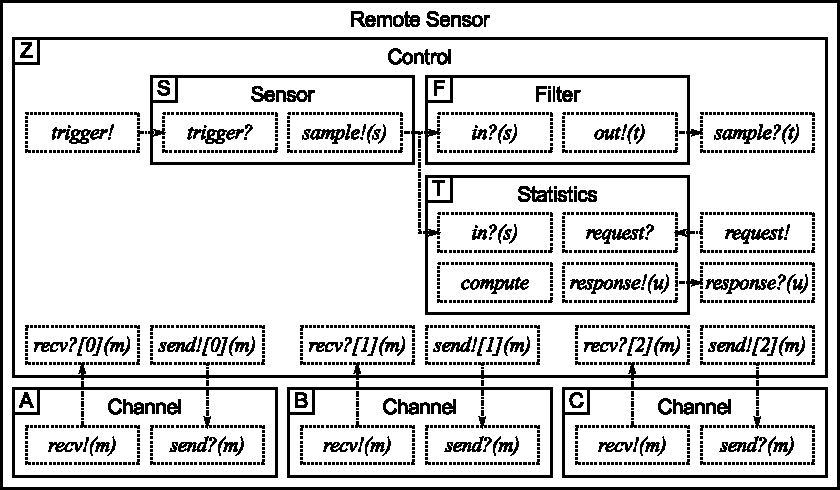
\includegraphics[width=\columnwidth]{example1}
\caption{Example remote sensor system.}
\label{example1}
\end{figure}

\paragraph*{Example.}
Figure~\ref{example1} depicts a remote sensor system as a composition of automata using a scheme similar to Figure~\ref{sys_model} where parameters are given in brackets after the action name, e.g., \emph{recv?[0](m)}.
The Remote Sensor automaton consists of the Control automaton Z and three Channel automata A, B, and C representing three network connections.
The Control automaton Z consists of the Sensor automaton S, the Filter automaton F, and the Statistics automaton T.
The Control automaton C starts the sampling process with the uv-up output $Z.trigger!$.
The uv-up input $S.trigger?$ is executed atomically with $Z.trigger!$ due to the binding $(Z.trigger!, S.trigger?)$.
When the sampling process is complete, the v-up output $S.sample!(s)$ distributes the sample to the Filter F and Statistics component T via the $(S.sample!(s), F.in?(s))$ and $(S.sample!(s), T.in?(s))$ bindings.
Note that $S.sample!(s)$, $F.in?(s)$, and $T.in?(s)$ all agree on the type of the sample $s$.
The Filter automaton F passes the filtered sample to the Control automaton Z via the $(F.out!(t), Z.sample?(t))$ binding.
The Statistics automaton T calculates the statistics incrementally using the up internal $T.compute$.
The statistics can be polled by the Control automaton Z by issuing a request via the $(Z.request!, T.request?)$ binding and then receiving a response via the $(T.response!(u), Z.response?(u))$ binding.
The Control automaton Z contains a vp-output $Z.send![](m)$ and a vp-input $Z.recv?[](m)$ for sending and receiving network messages using the Channel automata A, B, and C.
The parameters 0, 1, and 2, are used to route messages to Channel automata A, B, and C respectively using the session idea mentioned previously.
Opportunities for concurrent execution exist for the remote sensor depicted in Figure~\ref{example1}.
The set of automata implied by $Z.trigger!$ is $\{Z, S\}$ while the set of automata implied by $T.compute$ is $\{T\}$.
Since the sets are disjoint, the two actions can be executed concurrently.
\fi

%% \subsection{Practical Considerations\label{practical}}

%% As a mathematical abstraction the I/O automata model is appropriate for modeling reactive asynchronous and concurrent systems.
%% However, it lacks certain features needed to develop real components.
%% This subsection introduces these features and lays the foundation for adding the dynamics discussed in Section~\ref{dynamics}.

%% The I/O automata model assumes that systems are composed of a finite or countably infinite number of automata~\cite{lynch1996distributed}.
%% Assuming a countably infinite number of participants allows properties of the systems to be stated in terms of an abstract quantity representing the number of members, e.g., $N$, and is reasonable because all real systems are composed of a finite number of members.
%% The set of interactions in the I/O automata model is also fixed since automata are statically composed.
%% Dynamic systems can be \emph{modeled} in that approach by assuming that only a subset of the all the automata that could possibly exist are actively participating in the system.
%% To use this technique, a flag is associated with each automaton indicating if it is active or inactive and external actions for activation and deactivation are defined~\cite{lynch1994atomic}.

%% \paragraph*{Limitations of the static model.}
%% While assuming a fixed number of automata is reasonable for modeling, assuming a fixed number of automata for a real system may result in either over-provisioning or inflexibility.
%% To develop a component based on the static I/O automata model, a developer must choose a concrete value for the abstract quantity $N$.
%% System resources are wasted if the actual number of participants is much smaller than $N$.
%% If the number of participants is greater than $N$, then the system cannot respond to certain situations even though resources might be available.
%% Thus, the techniques for \emph{modeling} a dynamic system of I/O automata are not necessarily appropriate for \emph{implementing} a dynamic system of I/O automata.
%% %% Consequently, we add the ability to deal with a dynamic set of automata and interactions.

%% To illustrate, let a system $S=(A,B)$ be a pair consisting of a set of automata $A$ and a set of bindings $B$.
%% The I/O automata model assumes that $S$ and therefore $A$ and $B$ are both fixed, so that dynamics must be \emph{simulated} via the manipulation of activation flags.

\paragraph*{Support for dynamic systems.}
The I/O automata model assumes that systems are composed of a finite or countably infinite number of automata~\cite{lynch1996distributed} and models dynamic systems by activating and deactivating automata as appropriate~\cite{lynch1994atomic}.
While appropriate for modeling, this assumption is not conducive to building flexible and efficient systems because it requires \emph{a priori} bounds on all resources.
To address the limitations of the static representation of dynamic systems, ioa++ provides architectural support for dynamic systems by separating the concerns of \emph{enacting} versus \emph{initiating} actions for managing dynamics into distinct \emph{system} and \emph{base} automata respectively.
We define four \emph{system actions} for managing dynamic systems of automata: \emph{create}, \emph{bind}, \emph{unbind}, and \emph{destroy}.
The \emph{create} action allows an automaton to create a child automaton.
The \emph{bind} action allows an automaton to associate an input action with an output action while the \emph{unbind} action allows an automaton to dissociate an input action from an output action.
The \emph{destroy} action allows an automaton to destroy a child automaton and all bindings associated with it (recursively).

\begin{figure*}
\center
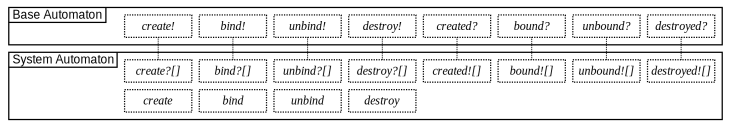
\includegraphics[width=\textwidth]{system_action}
\caption{System automaton and actions.}
\label{system_action}
\end{figure*}
% A dynamic system implies that the system $S$ must be dependent on time $t$ as a function of the number of actions that have been executed by $t$.
% Thus, $S_{t+1}$ need not be equal to $S_{t}$.
% A \emph{system action} is an action that \emph{can} change the system $S$.
% The set of automata $A$ and set of bindings $B$ are managed by the \emph{system automaton} which represents the run-time system.
As Figure~\ref{system_action} illustrates, the system automaton provides: parameterized input actions for receiving requests to create, bind, unbind, and destroy automata; internal actions for evaluating and enacting system action requests; and corresponding parameterized output actions for returning responses to system action requests.
(Parameterized actions are indicated with [].)
The base automaton provides output actions that trigger requests to create, bind, unbind, and destroy automata, along with
input actions to receive the results.
User-defined component automata (i.e., \emph{user automata}) inherit from the base automaton, which as we describe in Section~\ref{framework_architecture} is implemented in ioa++ as a C++ class. 
Each user automaton is thus composed (not bound) with the system automaton and inherits output actions for requesting system actions and input actions for receiving the results of system actions.

%% Let $A$ be the set of automata that exist where each element in $A$ is a pair $(p, a)$ where $p$ is the parent of $a$.
%% Let $B$ be the set of bindings that exist where each element in $B$ is a tuple $(w, o_a, o_n, o_p, i_a, i_n, i_p)$ where $w$ is the automaton that owns the binding, $o_a$ is the output automaton, $o_n$ is the name of the output action, $o_p$ is the parameter of the output action, $i_a$ is the input automaton, $i_n$ is the name of the input action, and $i_p$ is the parameter of the input action.
%% Define the predicate $exists (a) = \langle \exists p, q : (p, q) \in A :: q = a\rangle$ that is true when automaton $a$ exists, i.e., has a parent\footnote{The root automaton's parent is the special symbol $\perp$.}.
%% Define the predicate $existsb (a) = \langle \exists a : (w, o_a, o_n, o_p, i_a, i_n, i_p) \in B :: a = w \lor a = o_a \lor a = i_a \rangle$ that is true when automaton $a$ appears somewhere in $B$.
%% We define the create operation as the Hoare triple $\{exists (p) \land \lnot exists (a)\} \quad create(a)_p \quad \{(p,a) \in A\}$ which says that the parent automaton $p$ can create automaton $a$ if $p$ exists and $a$ does not exist.
%% The destroy operation can be defined $\{(p,a) \in A\} \quad destroy(a)_p \quad \{(p,a) \notin A \land \lnot existsb(a)\}$ which says that in order to destroy $a$ and remove all bindings associated with $a$, $p$ must be the parent of $a$.
%% Define the predicate $free (a, n, p) = \langle \forall w, o_a, o_n, o_p, i_a, i_n, i_p : (w, o_a, o_n, o_p, i_a, i_n, i_p) \in B :: \lnot (i_a = a \land i_n = n \land i_p = p) \rangle$ that is true when the input action argument is not bound.
%% Define the predicate $involved (o, n, p, i) = \langle \exists w, o_a, o_n, o_p, i_a, i_n, i_p : (w, o_a, o_n, o_p, i_a, i_n, i_p) \in B :: o_a = o \land o_n = n \land o_p = p \land i_a = i \rangle$ that is true when automaton $o$'s output action $(n, p, i)$ is bound to some input action in automaton $i$.
%% The bind operation can be defined $\{exists (w) \land exists (o_a) \land exists (i_a) \land free (i_a, i_n, i_p) \land \lnot involved(o_a, o_n, o_p, i_a) \land o_a \neq i_a \} \quad bind (w, o_a, o_n, o_p, i_a, i_n, i_p) \quad \{(w, o_a, o_n, o_p, i_a, i_n, i_p) \in B\}$ which says that in order for the binding to succeed the owner $w$ exists, automaton $o_a$ exists, automaton $i_a$ exists, the input action $(i_a, i_n, i_p)$ must not be bound, the output action $(o_n, o_p)$ of automaton $o_a$ cannot be bound to an input action in automaton $i_a$, and the automata $o_a$ and $i_a$ cannot be the same.
%% The precondition for $bind$ is same as the binding rules derived in Section~\ref{system_model} augmented with existence tests for the owner, output automaton, and input automaton.
%% The unbind operation is similar to destroy: $\{(w, o_a, o_n, o_p, i_a, i_n, i_p) \in B\} \quad unbind (w, o_a, o_n, o_p, i_a, i_n, i_p) \quad \{(w, o_a, o_n, o_p, i_a, i_n, i_p) \notin B\}$.

% I didn't do more complex transactions, i.e., create-and-bind, because its not clear how it fails.
% Are partial successes allowed?
% Furthermore, such  transactions can be arbitrarily complex which does not bode well for efficiency.

\paragraph*{Binding predicates.}
Consider a simple system consisting of two automata where automaton A reliably transfers messages to automaton B.
In a dynamic system, one cannot guarantee that the message will be received because there is no way to determine if the output action producing the message is bound to the input action receiving the message.
Since we can guarantee that the set of binding does not change during the execution of an action, we allow automata to query the current set of bindings using a \emph{binding predicate}.
Binding predicates are typically used the precondition of output actions to guarantee delivery.
